% \documentclass{article}
\documentclass{ctexart}

\usepackage{graphicx}
\usepackage{amsmath}
\usepackage{amssymb}
\usepackage{amsthm}
\usepackage{BOONDOX-cal}
\usepackage{subfigure}
\usepackage{url}
\usepackage{float}
\CJKfamily{song}
% \setCJKfamilyfont{song}
\CTEXsetup[format={\Large\bfseries}]{section}

% \newtheorem{corollary}{推论}[section]
\newtheorem{corollary}{推论}
\newtheorem{theorem}{定理}

% \setmonofont{Consolas}
\usepackage{listings}
\usepackage{color,xcolor}
\setlength{\parindent}{0pt}

\title{作业四:Mandelbrot Set 的生成和探索}


\author{常笑 \\ 数学与应用数学 \\ 3190102223 }

\begin{document}

\maketitle

\begin{abstract}
本文主要说明了Mandelbrot Set的生成的原理和所依赖的发散性定理,并使用c语言实现了Mandelbrot Set 的图片,同时研究了不同的迭代上限对最终生成图片的影响。
\\
% \noindent{\textbf{关键字:} }
\end{abstract}
\thispagestyle{empty}

\section{引言}
\indent 在对现实世界的探索和研究当中,我们总是设想世界万物是连续的,但这已被量子力学所推翻,而在用数学模型来描述现实中的三维物体,我们也总是认为它的边界是几乎处处光滑的,这是简洁,有秩序的,但是分形学的研究则推翻了这一假定,以一种混沌夹杂有序的方式反映现实中的结构。
\subsection{问题的背景介绍}
\indent 在利用牛顿法求解多项式的根时,我们通常没有关注于牛顿法对任意初始点的收敛性,而是总取初始点足够接近多项式的一个根,这样牛顿法最终就会收敛到在该点附近的那个根,但是我们并没有办法确定所有的点是否都在牛顿法的迭代下收敛到一个解,如果将复平面上所有经过牛顿法迭代后最终收敛到多项式根的点染色,一个根对应一种颜色,我们可以得到对于多项式$P(z) = z^5 + z^2 - z + 1$的一张图\ref{1}\cite{3B1B_Mandelbrot_Set}。本质上牛顿迭代法是做$z_{n+1} = z_n - \frac{P(z_n)}{P^{'}(z_n)} = G(z_n)$,其中$G(z)$是一个有理多项式,当我们取$G(z) = z^2 + c$时,并从原点开始迭代,将迭代序列有界的$c$涂上一种颜色,其他的涂成别的颜色,我们就可以得到这样的一张图\ref{2}\\

\begin{figure}[h]
\centering
\subfigure[\label{1} newton pattern]
{
    \begin{minipage}[b]{.45\linewidth}
        \centering
        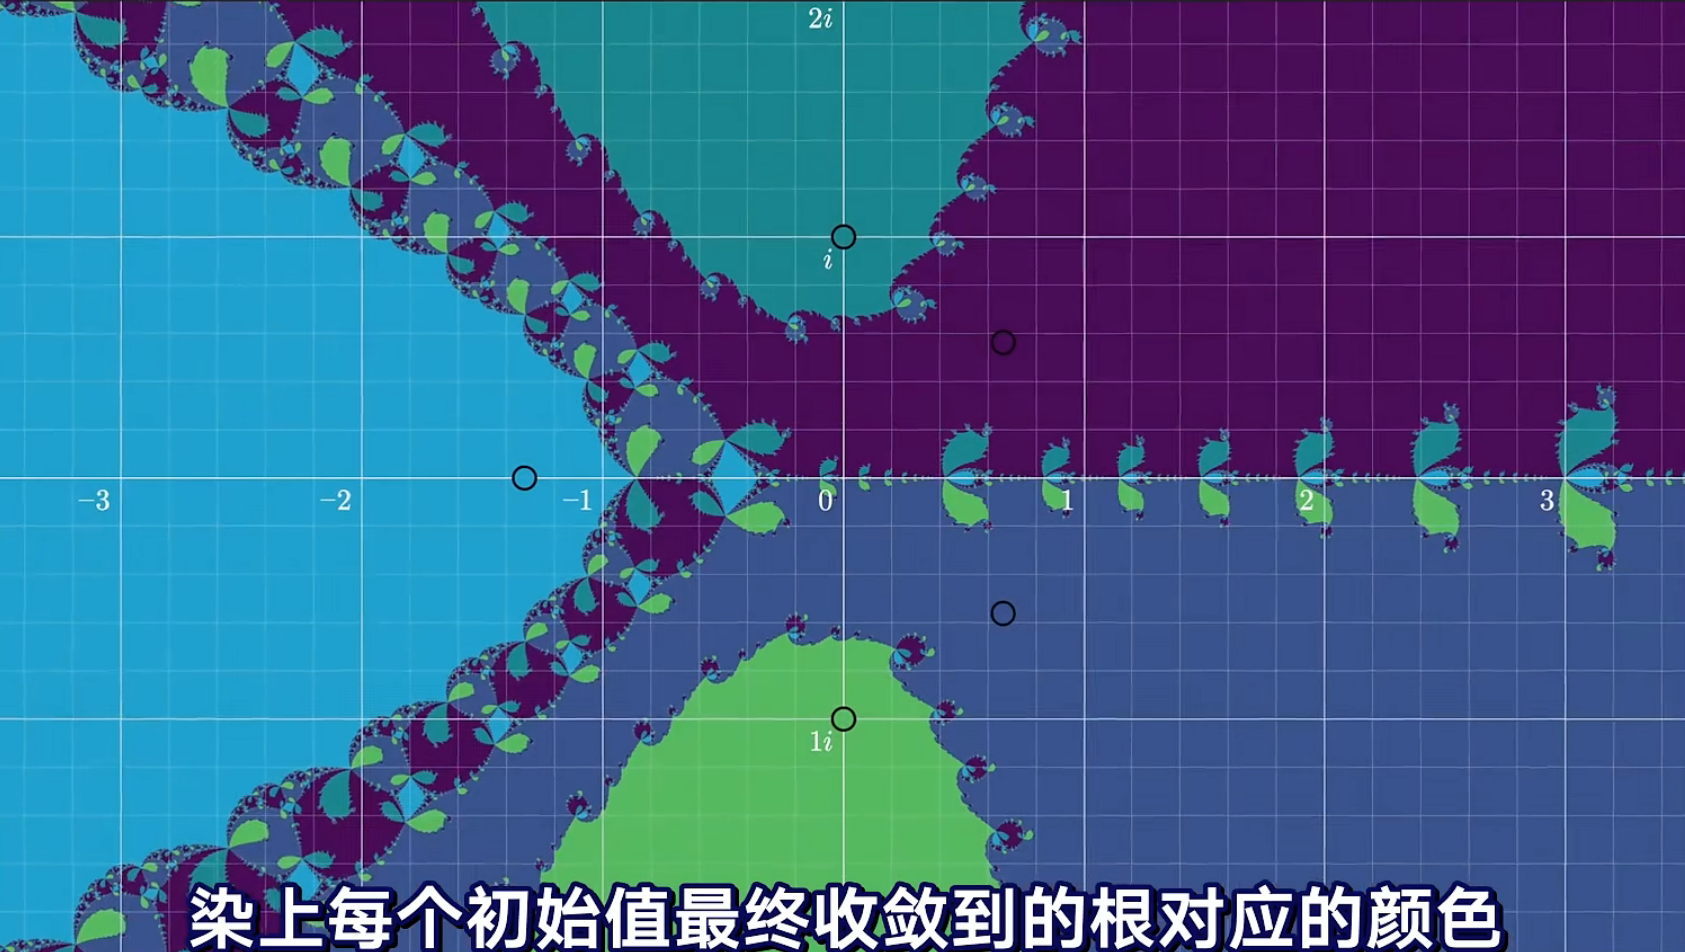
\includegraphics[width=5cm]{./examples/example.png}
    \end{minipage}
}
\subfigure[\label{2} Mandelbrot Set]
{
 	\begin{minipage}[b]{.45\linewidth}
        \centering
        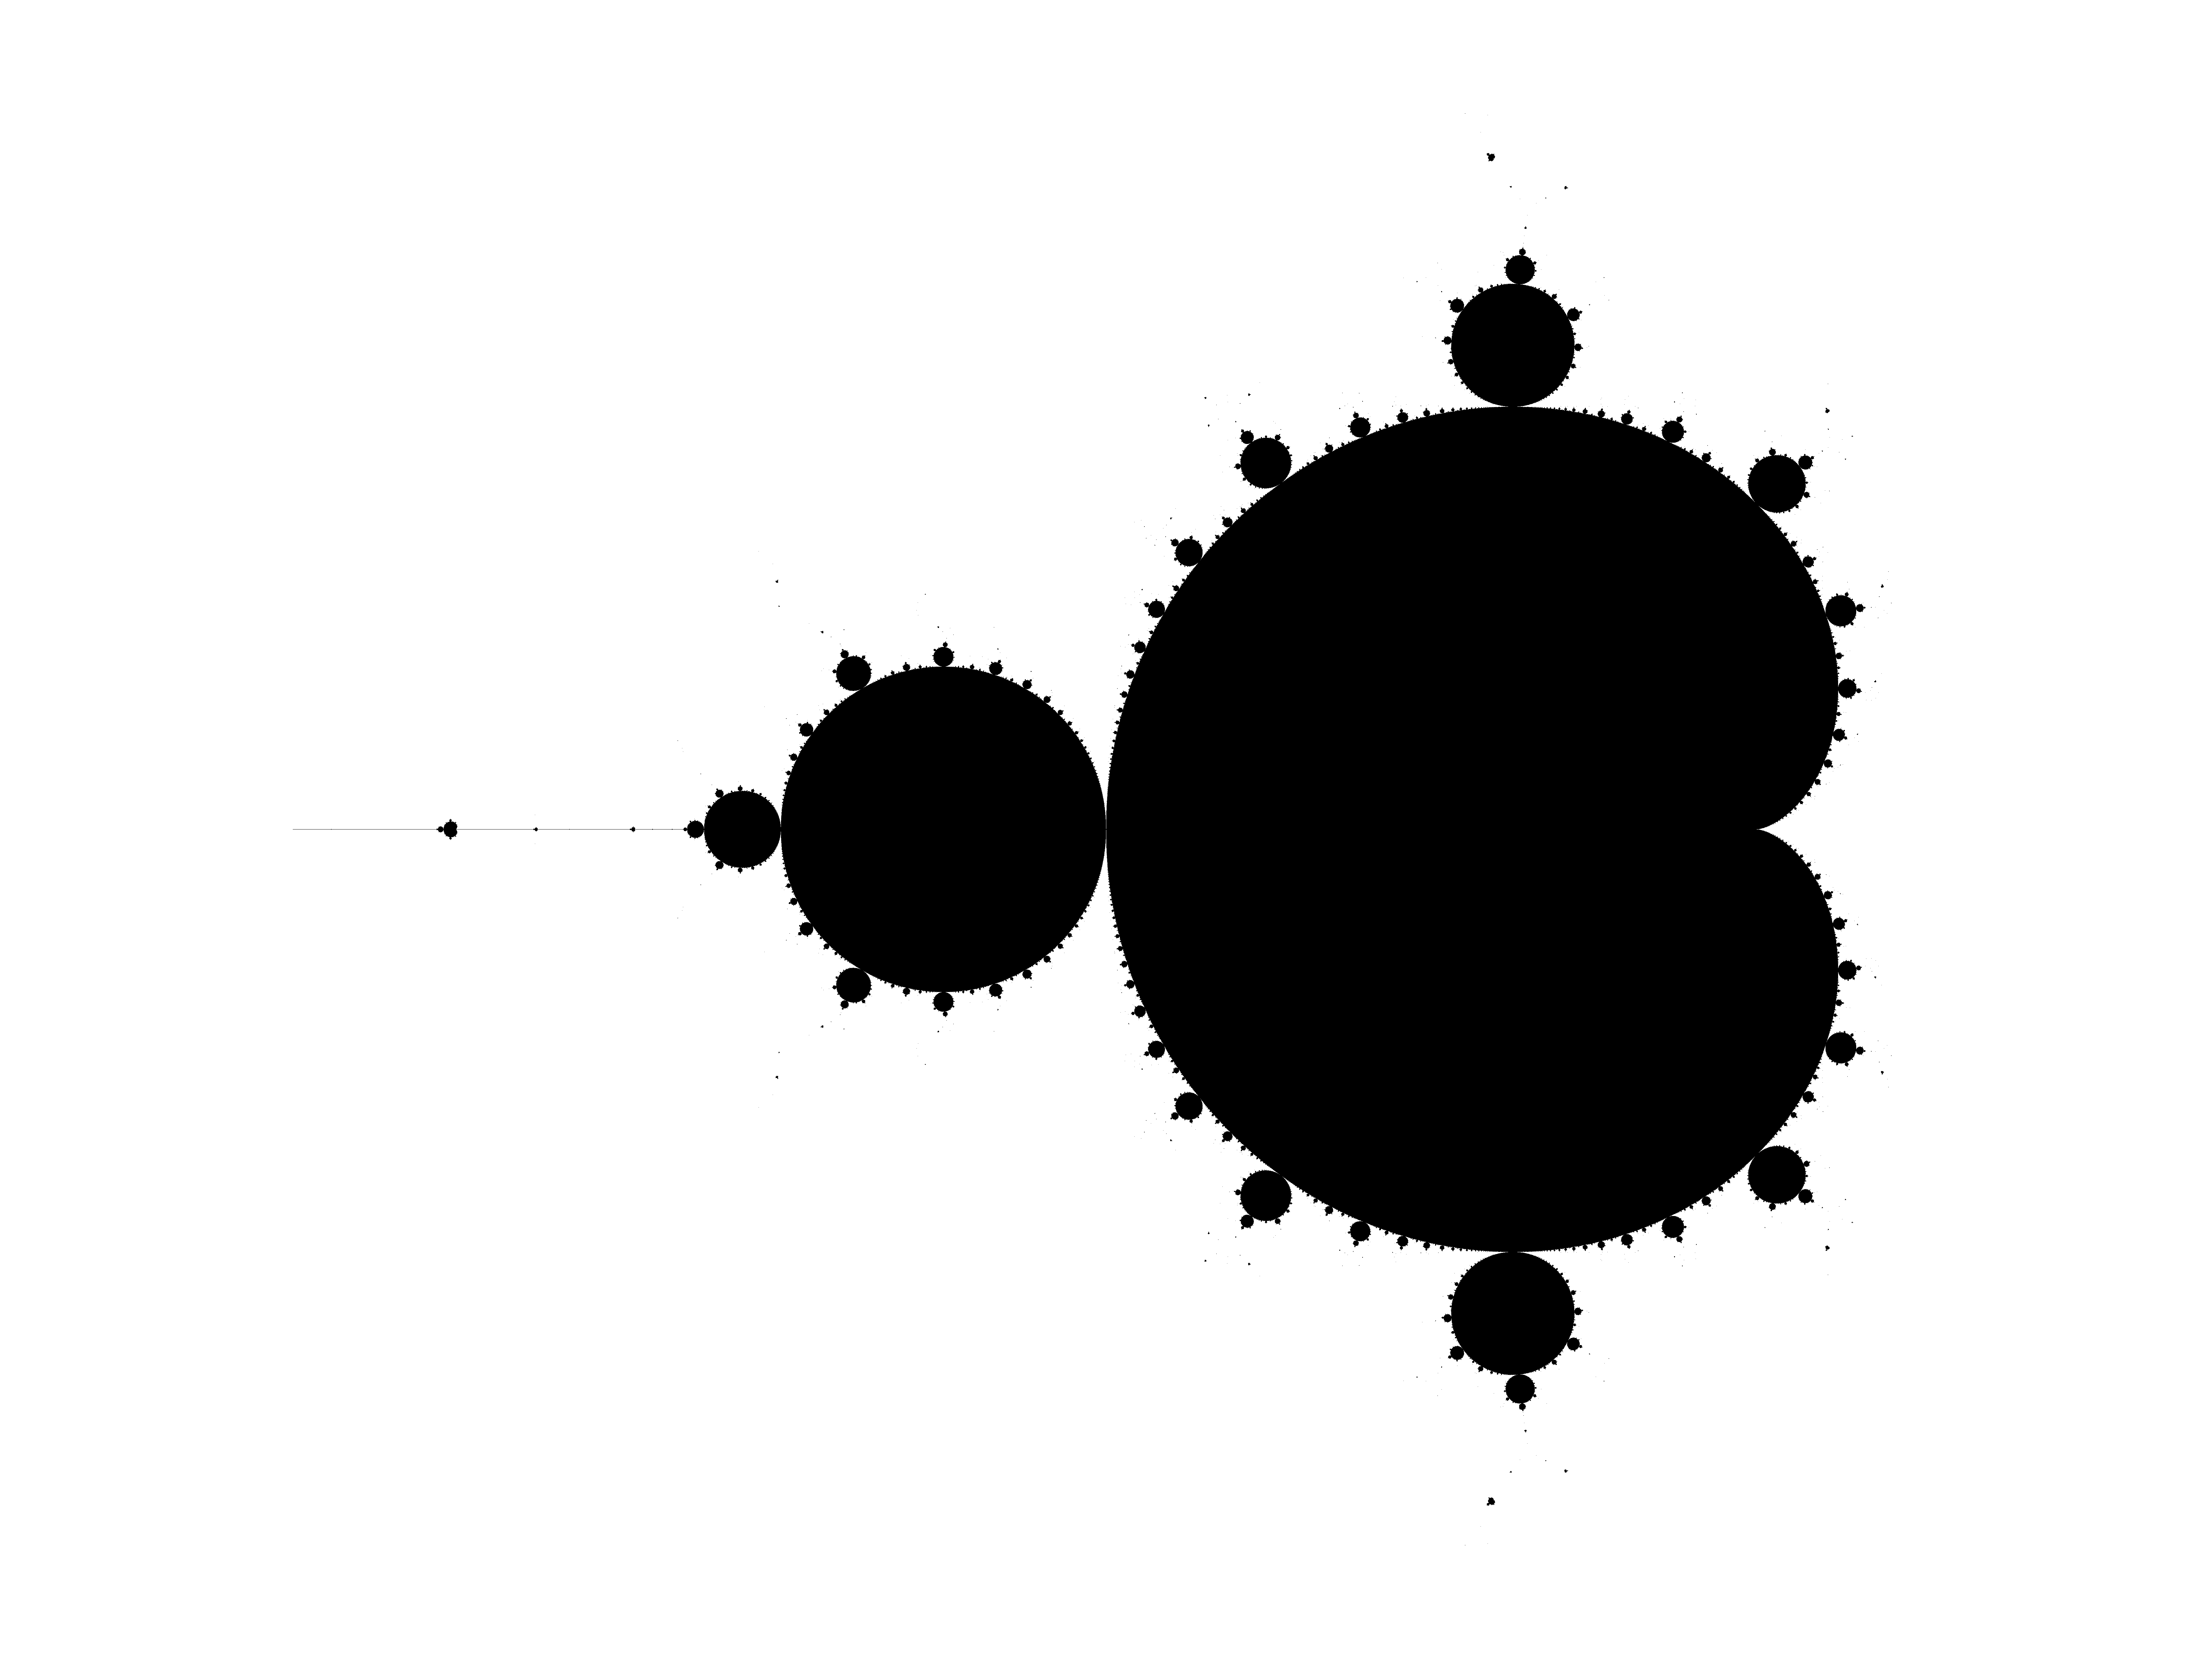
\includegraphics[width=5cm]{./examples/res_5000.png}
    \end{minipage}
}
\caption{}
\end{figure}

\indent 咋一看这两个图没有什么相关性,如果看多项式$P(z) = (z - 1)(z + 1)(z - \lambda)$,当$\lambda$取值使其中重心$\frac{\lambda}{3}$在牛顿法迭代法中趋向于循环时,将这个$\lambda$涂为黑色,那么在这个相应的图里放大后,可以找到与Mandelbrot Set相同的图案。\\
\indent 不过现在还有一个问题,上边的图\ref{1}是要确定每一个$c$对应的迭代序列是否收敛,需要一个相应的判定准则,这个判定准则就是我们能成功画出这一个图的关键。

\section{数学理论}
\indent 对于这一个判定准则,我们有下边定理:
\begin{theorem}[1]
	序列{$z_n,n=0,1,\dots,z_n \in \mathbb{C}$}满足$z_0 = 0, z_{n+1} = z_n^2 + c$,该序列有界当且仅当$\forall n \in \mathbb{N}$,有$|z_n| \le max\{2,|c|\}$
\end{theorem}
\begin{proof}
	:\\
	$\leftarrow$:由有界的定义易得。\\
	$\rightarrow$:反证法,若存在 $z_j$ 使得 $|z_j| > max\{2,|c|\}$ , 则有 $|z_j| = max\{2,|c|\} + \epsilon$ \\
	\indent 从而有 $|z_{j+1}| \ge |z_j|^2 - |c| \ge |z_j|^2 - |z_j| \ge (1 + \epsilon)|z_j|$\\
	\indent 因此 $|z_{j+k}| \ge (1 + \epsilon)^k|z_j|$,这说明序列无界。
\end{proof}
\begin{corollary}[2]
	序列{$z_n,n=0,1,\dots,z_n \in \mathbb{C}$}满足$z_0 = 0, z_{n+1} = z_n^2 + c$,该序列有界当且仅当$\forall n \in \mathbb{N}$,有$|z_n| \le 2$
\end{corollary}
\begin{proof}
	当 $|c| \le 2$ 时,这没有区别,当 $|c| > 2$ 时,我们有 $|z_2| = |c^2 + c| = |c + 1||c| > |c| = max\{2,|c|\}$,这满足上边定理的条件。
\end{proof}

\section{算法}
\indent 由上边的定理可知,确定一个序列是否是发散的,只需要看这一个序列当中是否有模长大于2的元素即可。伪代码如下:
\begin{lstlisting}[language = Python, numbers=left,breaklines=true,
         numberstyle=\tiny,keywordstyle=\color{blue!70},
         commentstyle=\color{red!50!green!50!blue!50},frame=shadowbox,
         rulesepcolor=\color{red!20!green!20!blue!20},basicstyle={\ttfamily\footnotesize}]
确定一个迭代上限 N
for 图中的像素点 p :
    令 c 为该像素点对应的复数
    令 z 为迭代序列,初始值为0
    for i = 1,2,...,N:
        z = z**2 + c
        if  z 的模长 > 2:
			设置该像素点的颜色为白色
			break
    else:
        设置该像素点的颜色为黑色
 \end{lstlisting}
 \section{数值算例}
\indent 由上边伪代码可知,实际画出的图像是近似的图,迭代次数上限会直接影响画出来的图案,设置迭代次数 N 分别为 20,40,100,400,5000时画出来的图像如图\ref{Two}。\\
\begin{figure}[H]
\centering
\subfigure[N=20]
{
    \begin{minipage}[b]{.3\linewidth}
        \centering
        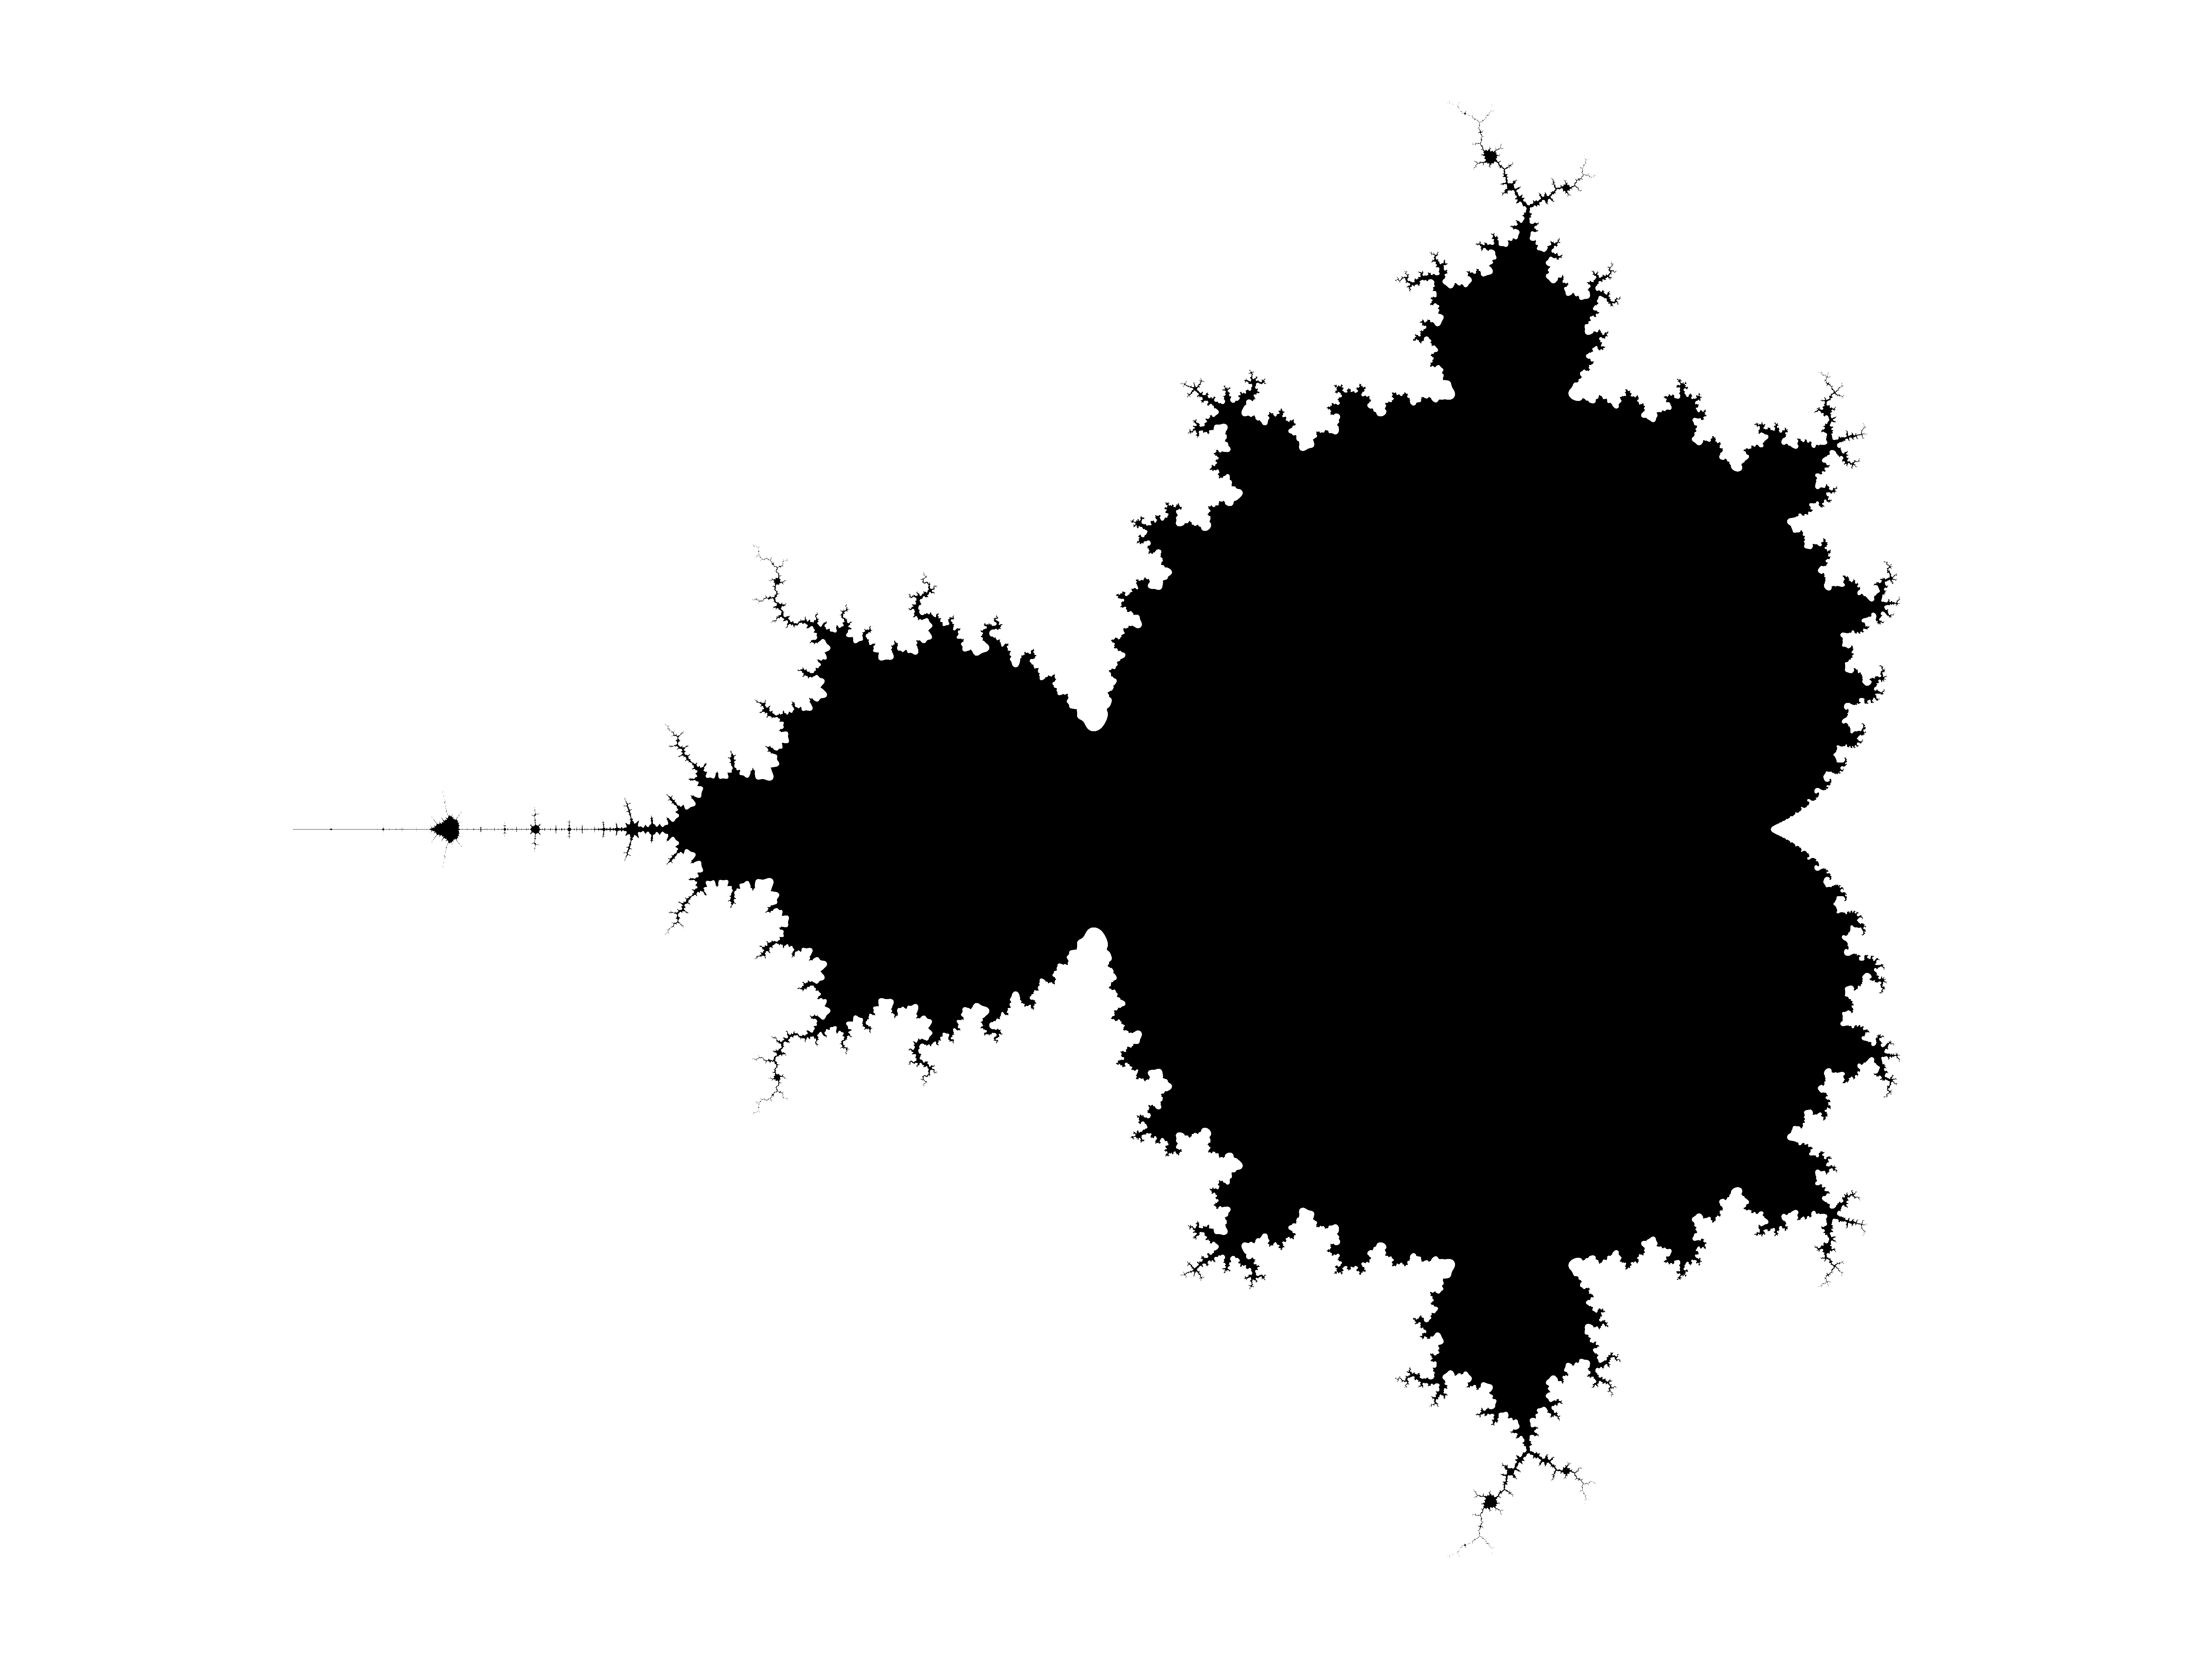
\includegraphics[width=3cm,height = 1.75cm]{./examples/res_20.png}
    \end{minipage}
}
\subfigure[N=40]
{
 	\begin{minipage}[b]{.3\linewidth}
        \centering
        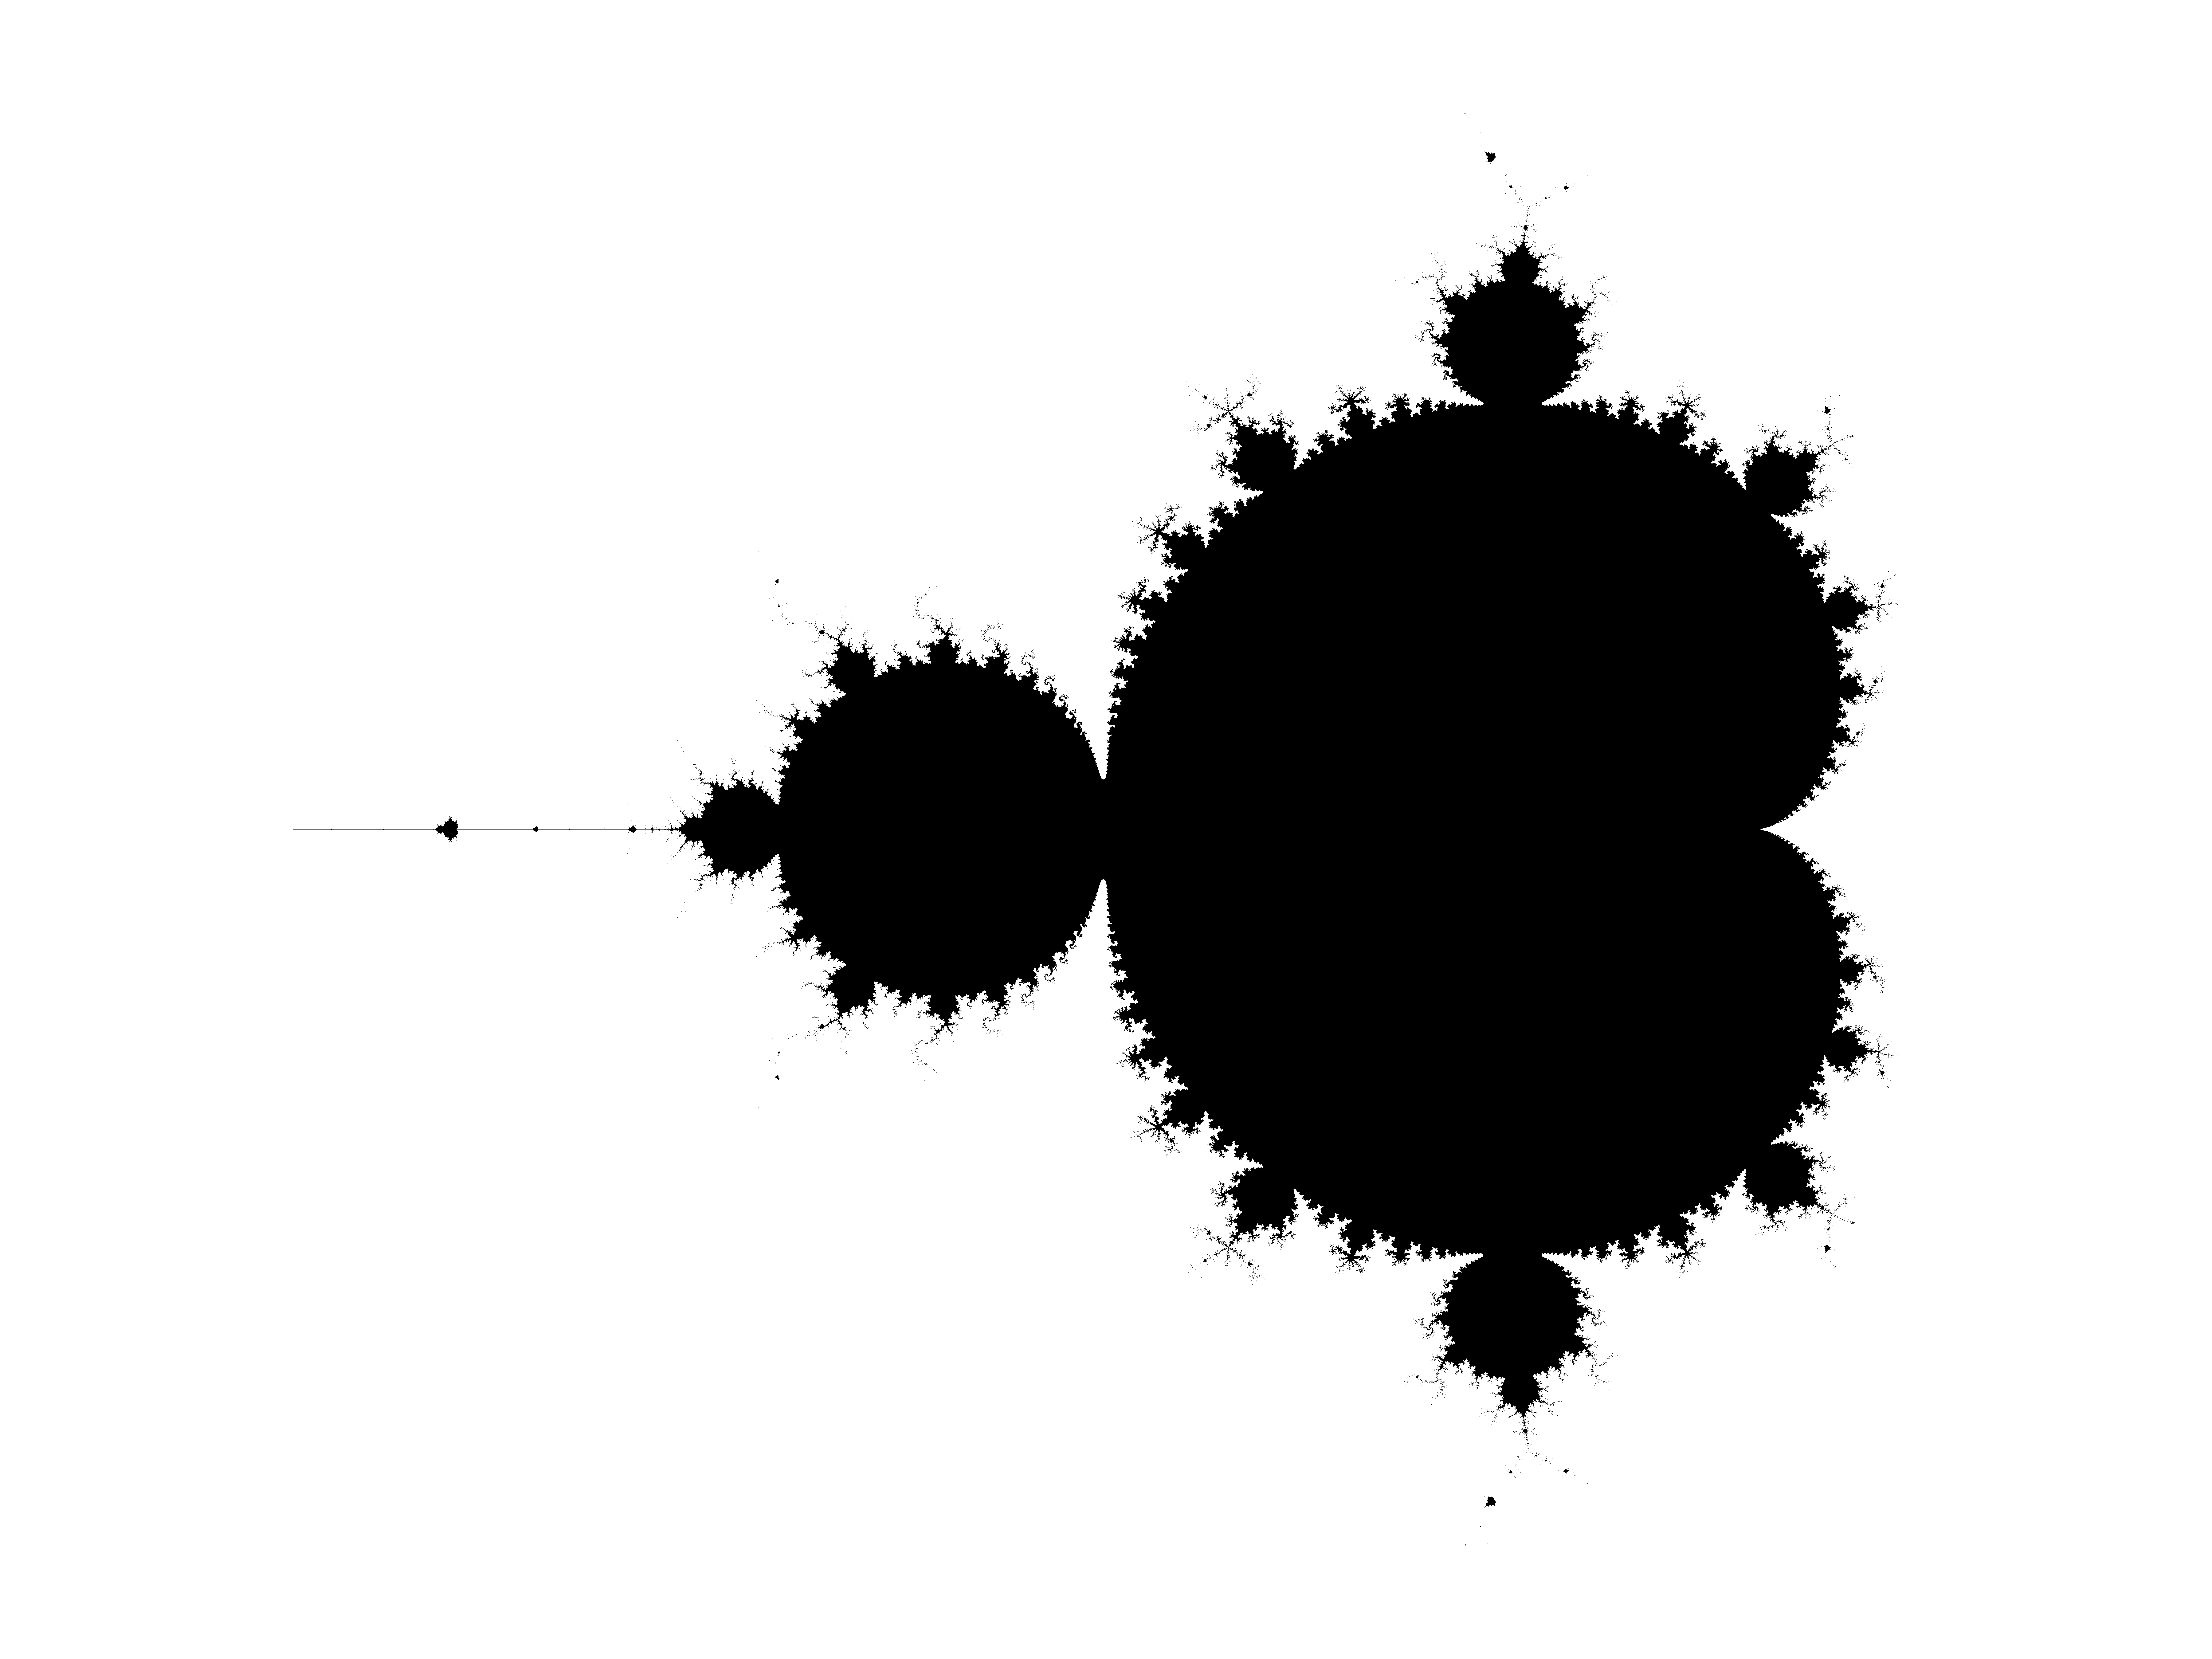
\includegraphics[width=3cm,height = 1.75cm]{./examples/res_40.png}
    \end{minipage}
}
\subfigure[N=100]
{
 	\begin{minipage}[b]{.3\linewidth}
        \centering
        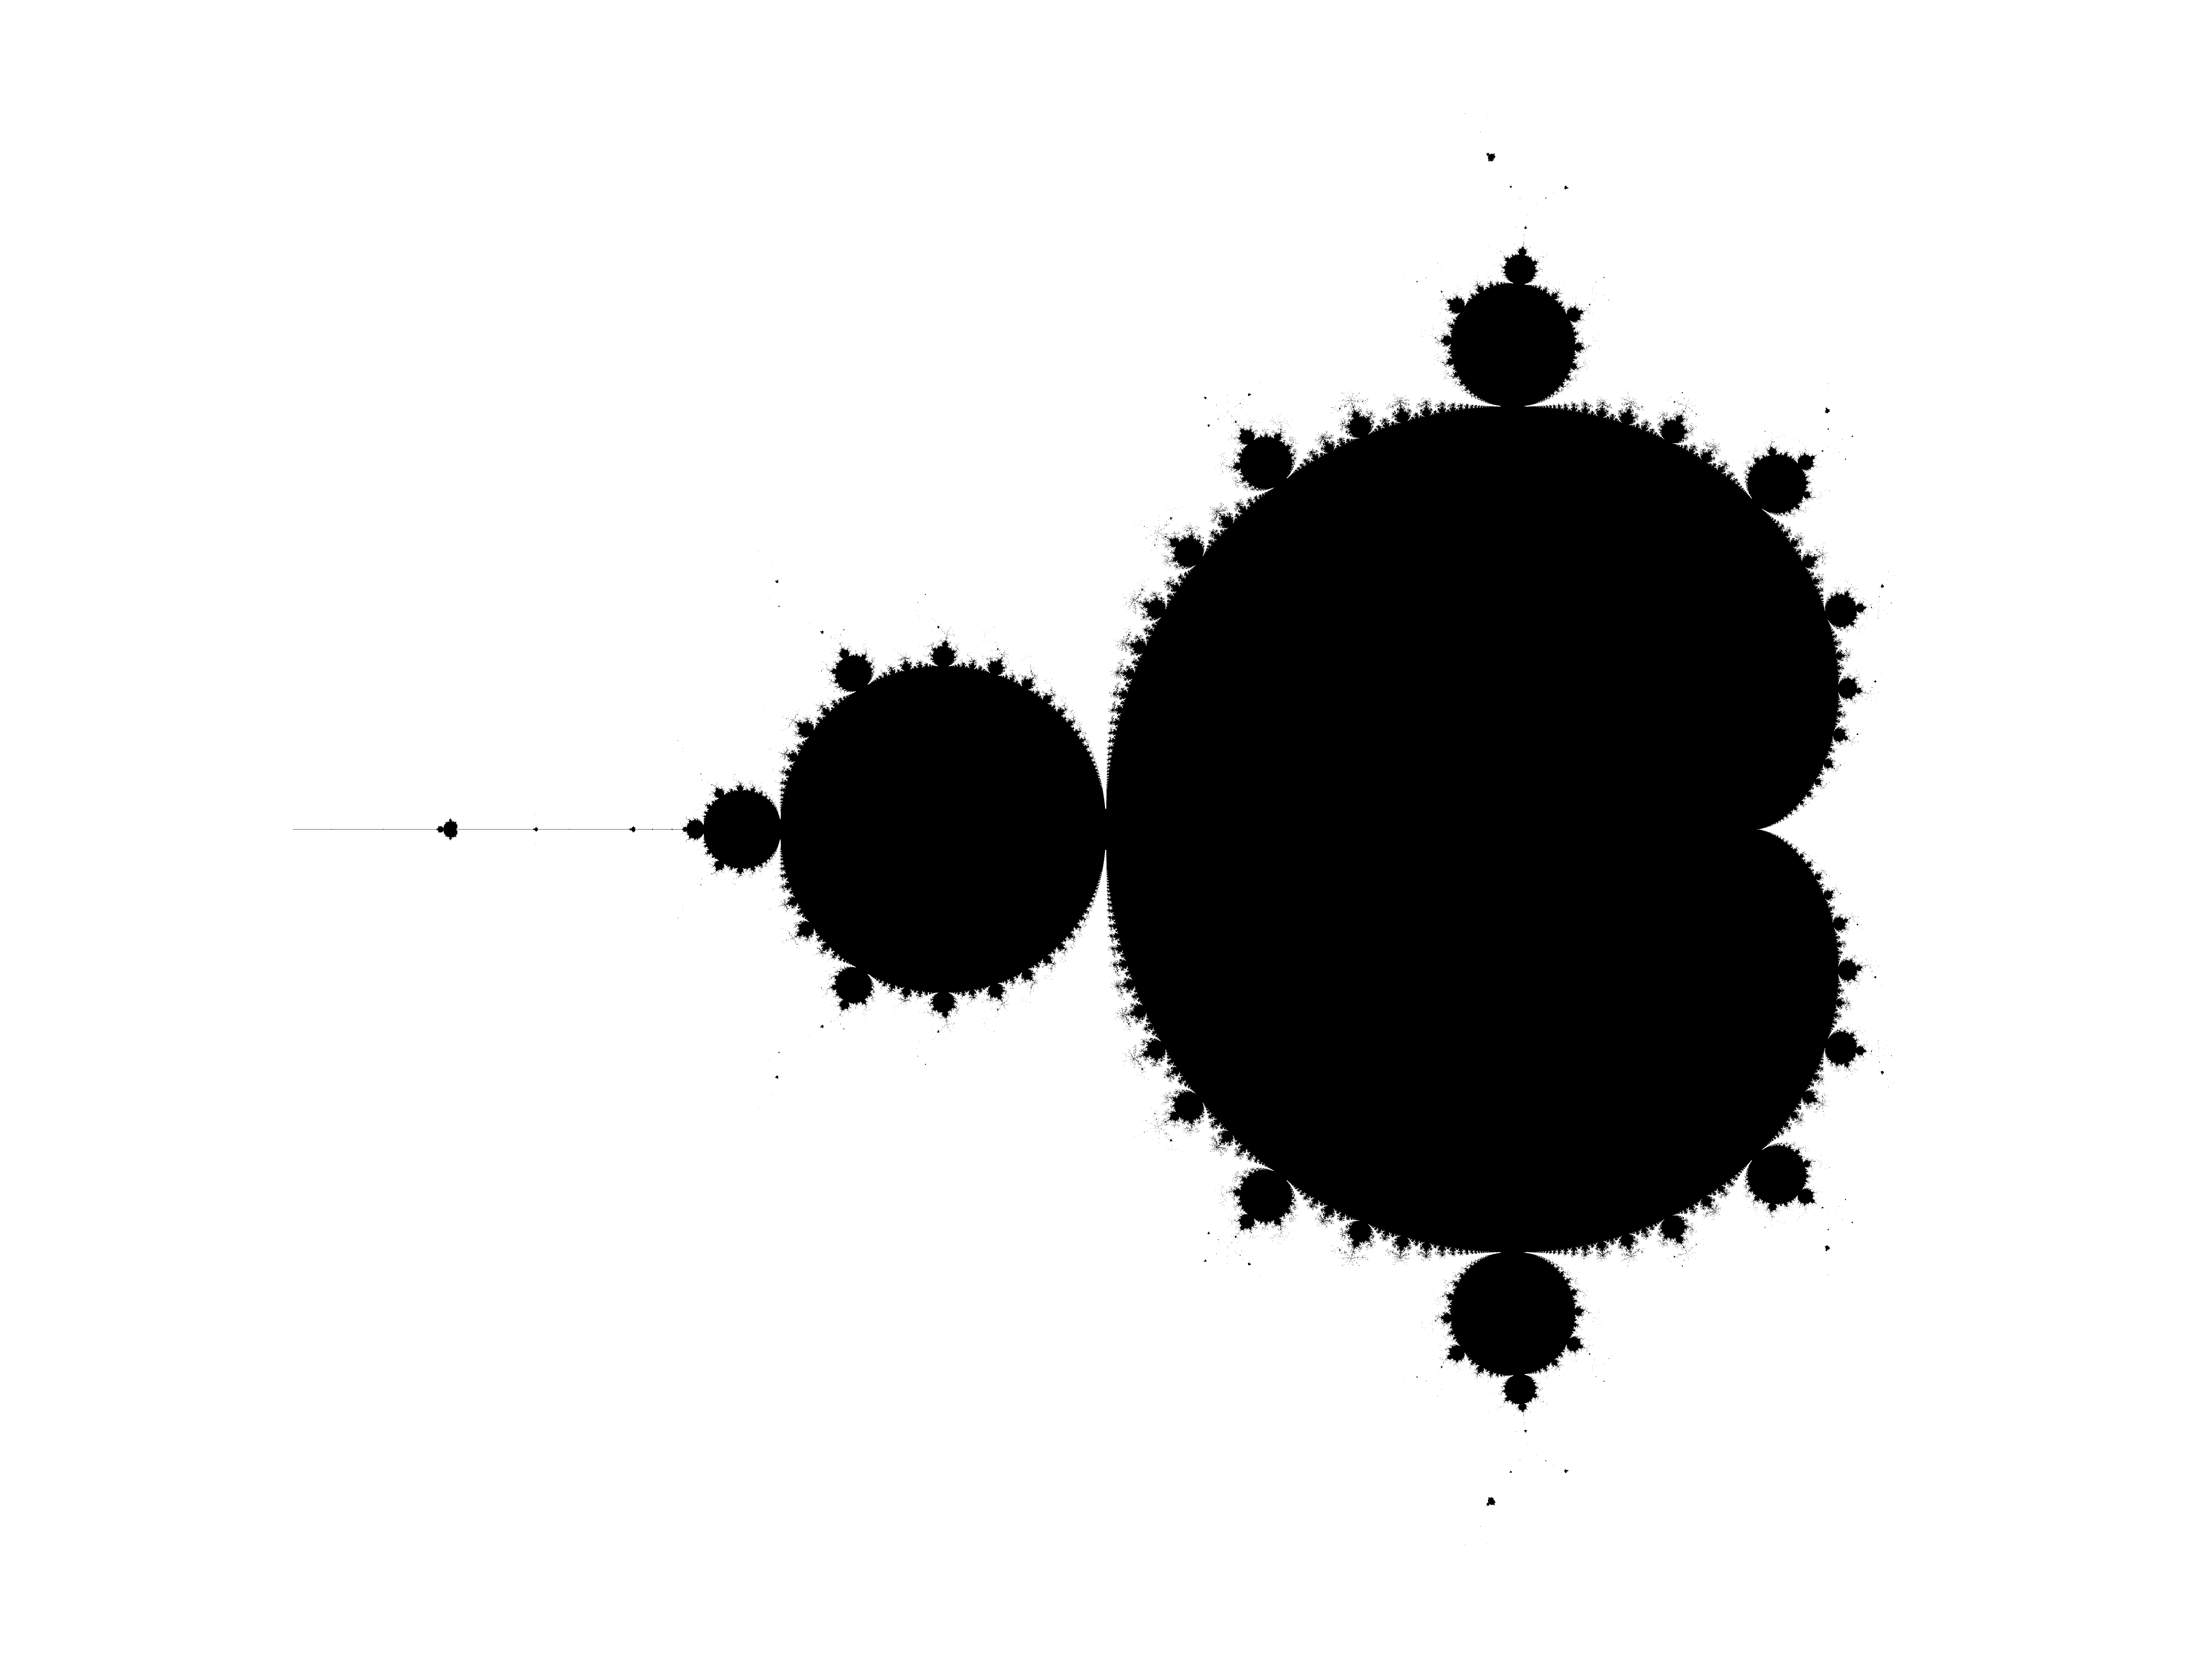
\includegraphics[width=3cm,height = 1.75cm]{./examples/res_100.png}
    \end{minipage}
}
\subfigure[N=400]
{
 	\begin{minipage}[b]{.45\linewidth}
        \centering
        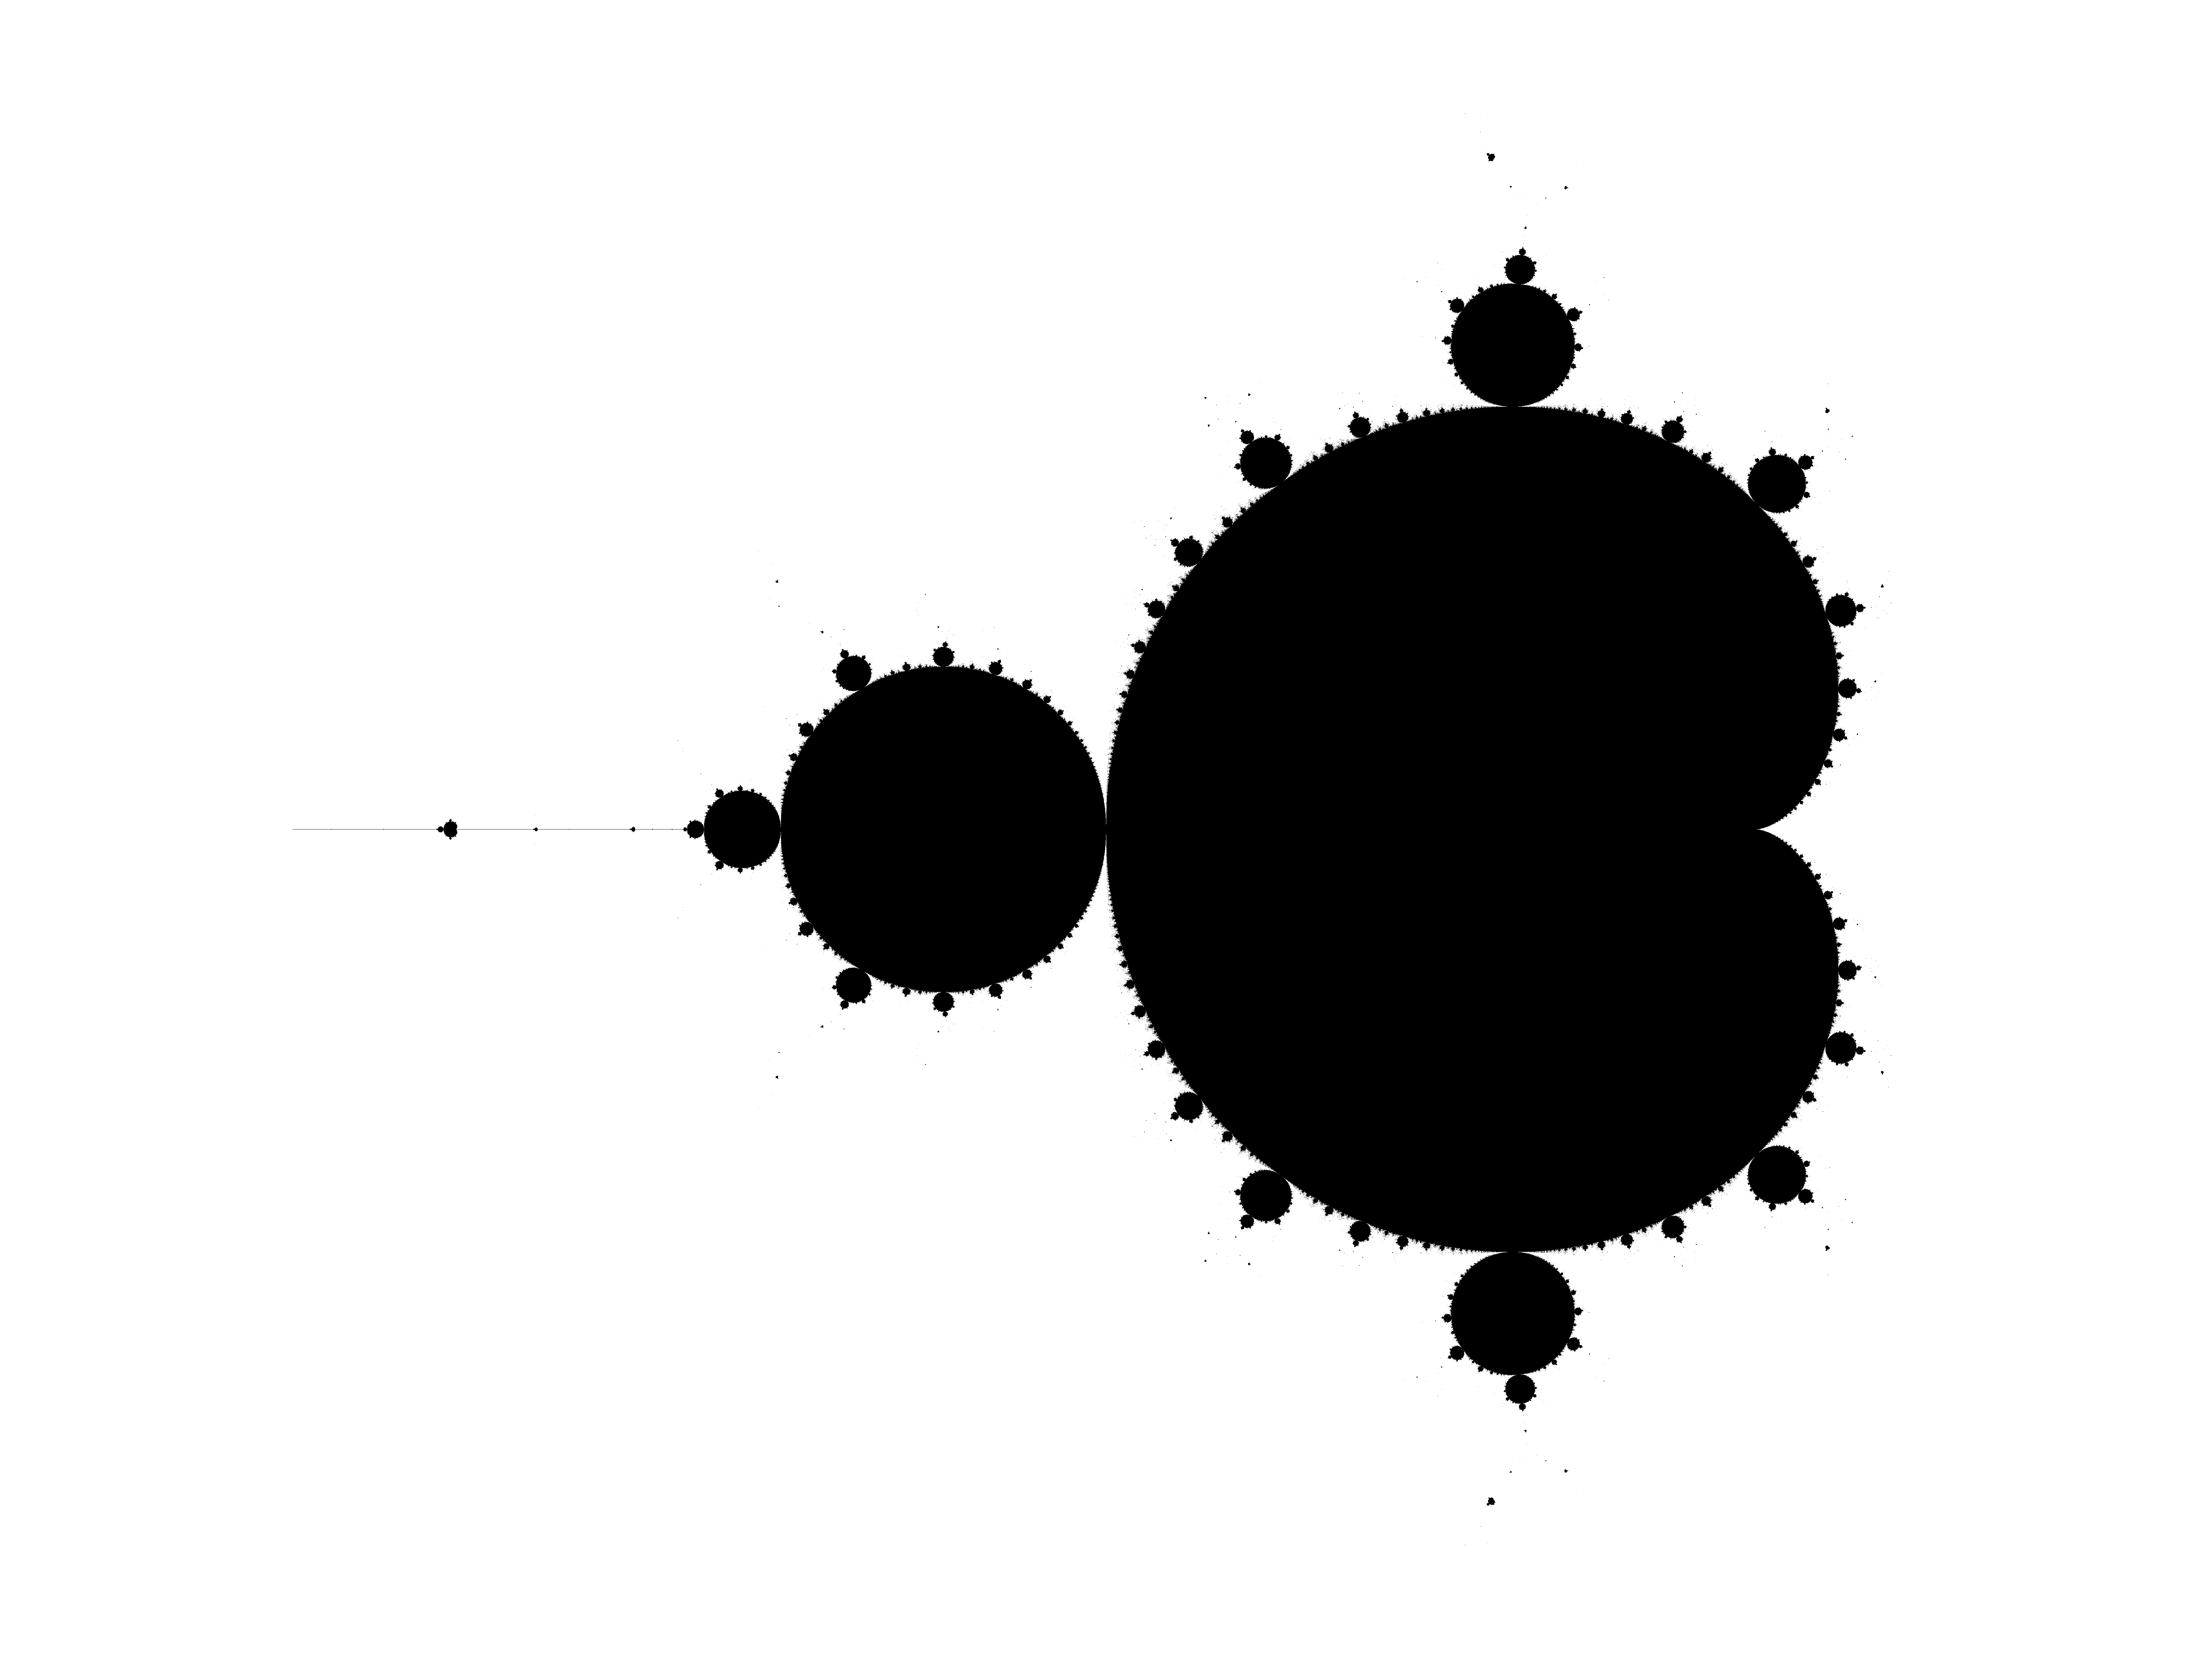
\includegraphics[width=5cm,height = 3.5cm]{./examples/res_400.png}
    \end{minipage}
}
\subfigure[N=5000]
{
 	\begin{minipage}[b]{.45\linewidth}
        \centering
        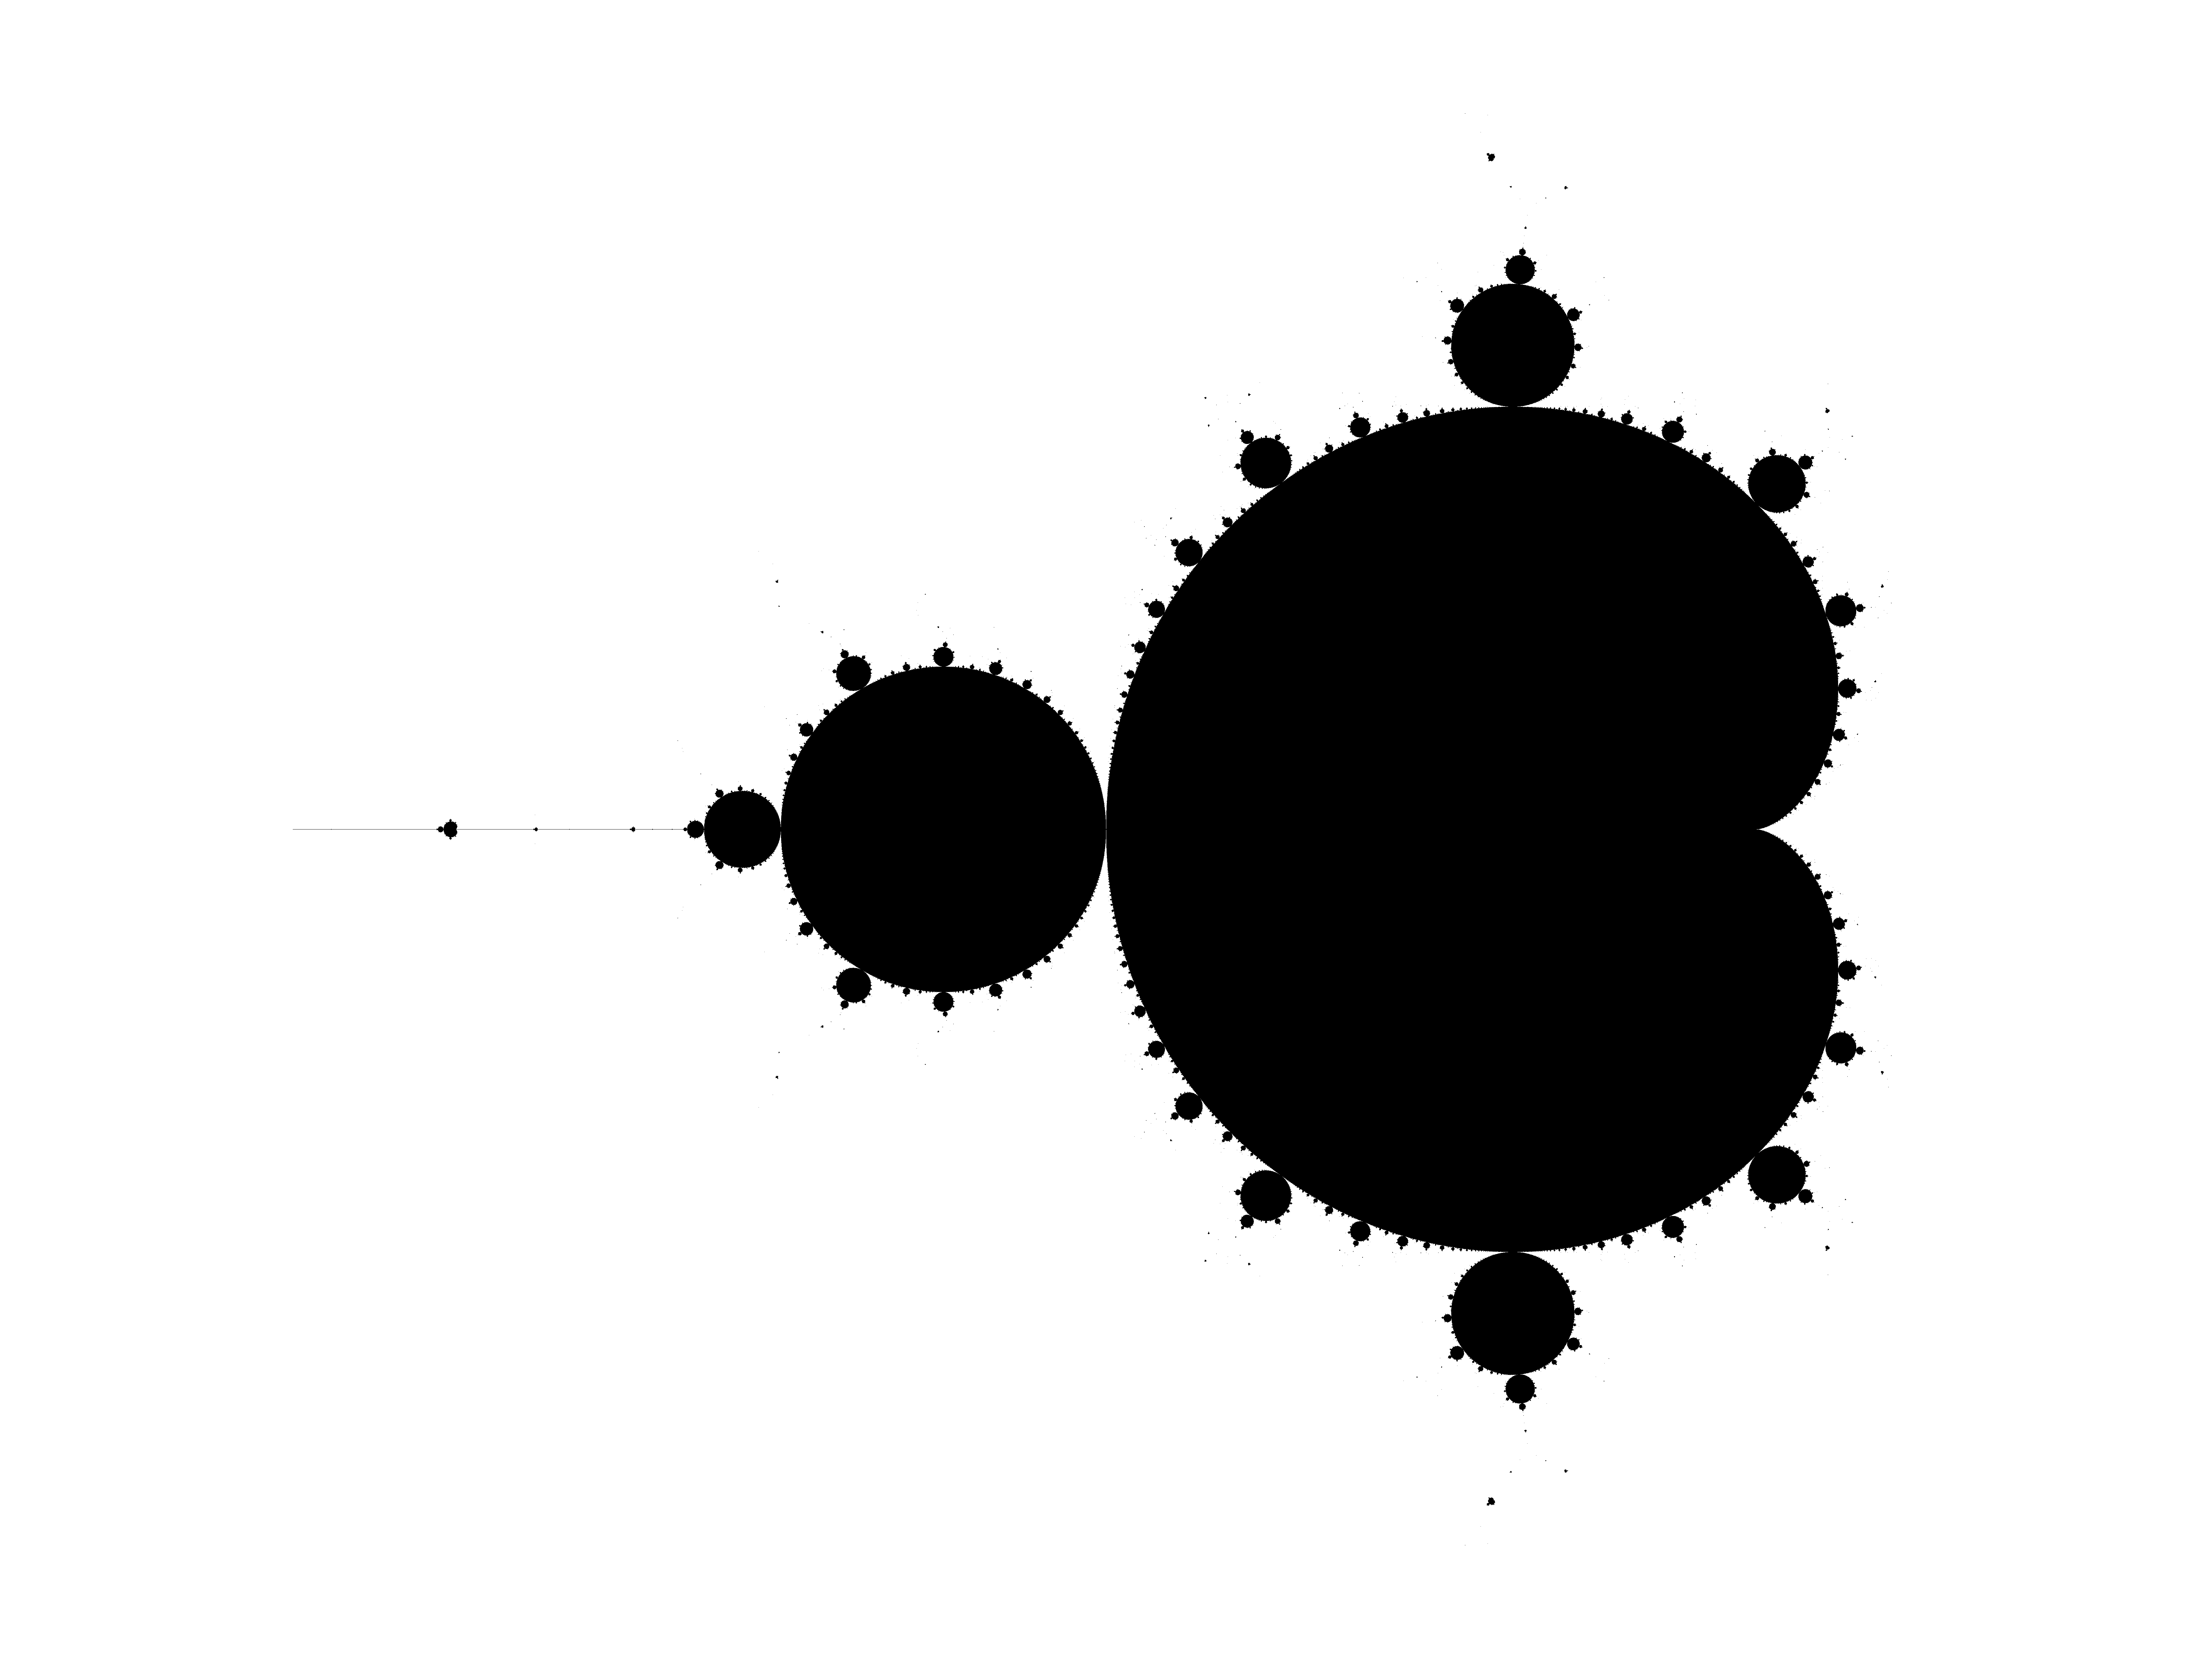
\includegraphics[width=5cm, height = 3.5cm]{./examples/res_5000.png}
    \end{minipage}
}
\caption{\label{Two}}
\end{figure}
\indent 可以看到迭代次数提升后图像外侧的细树枝样的图案逐渐变少,最终消失。如果我们根据每个点对应的序列被判定为发散的相应迭代次数来给整个图案上颜色,我们就可以得到下边的这样一张图案,图中可以看到有分层,这即相当于把设定 N 为各种值后将图片叠加起来的效果。\\
\begin{figure}[H]
\centering
	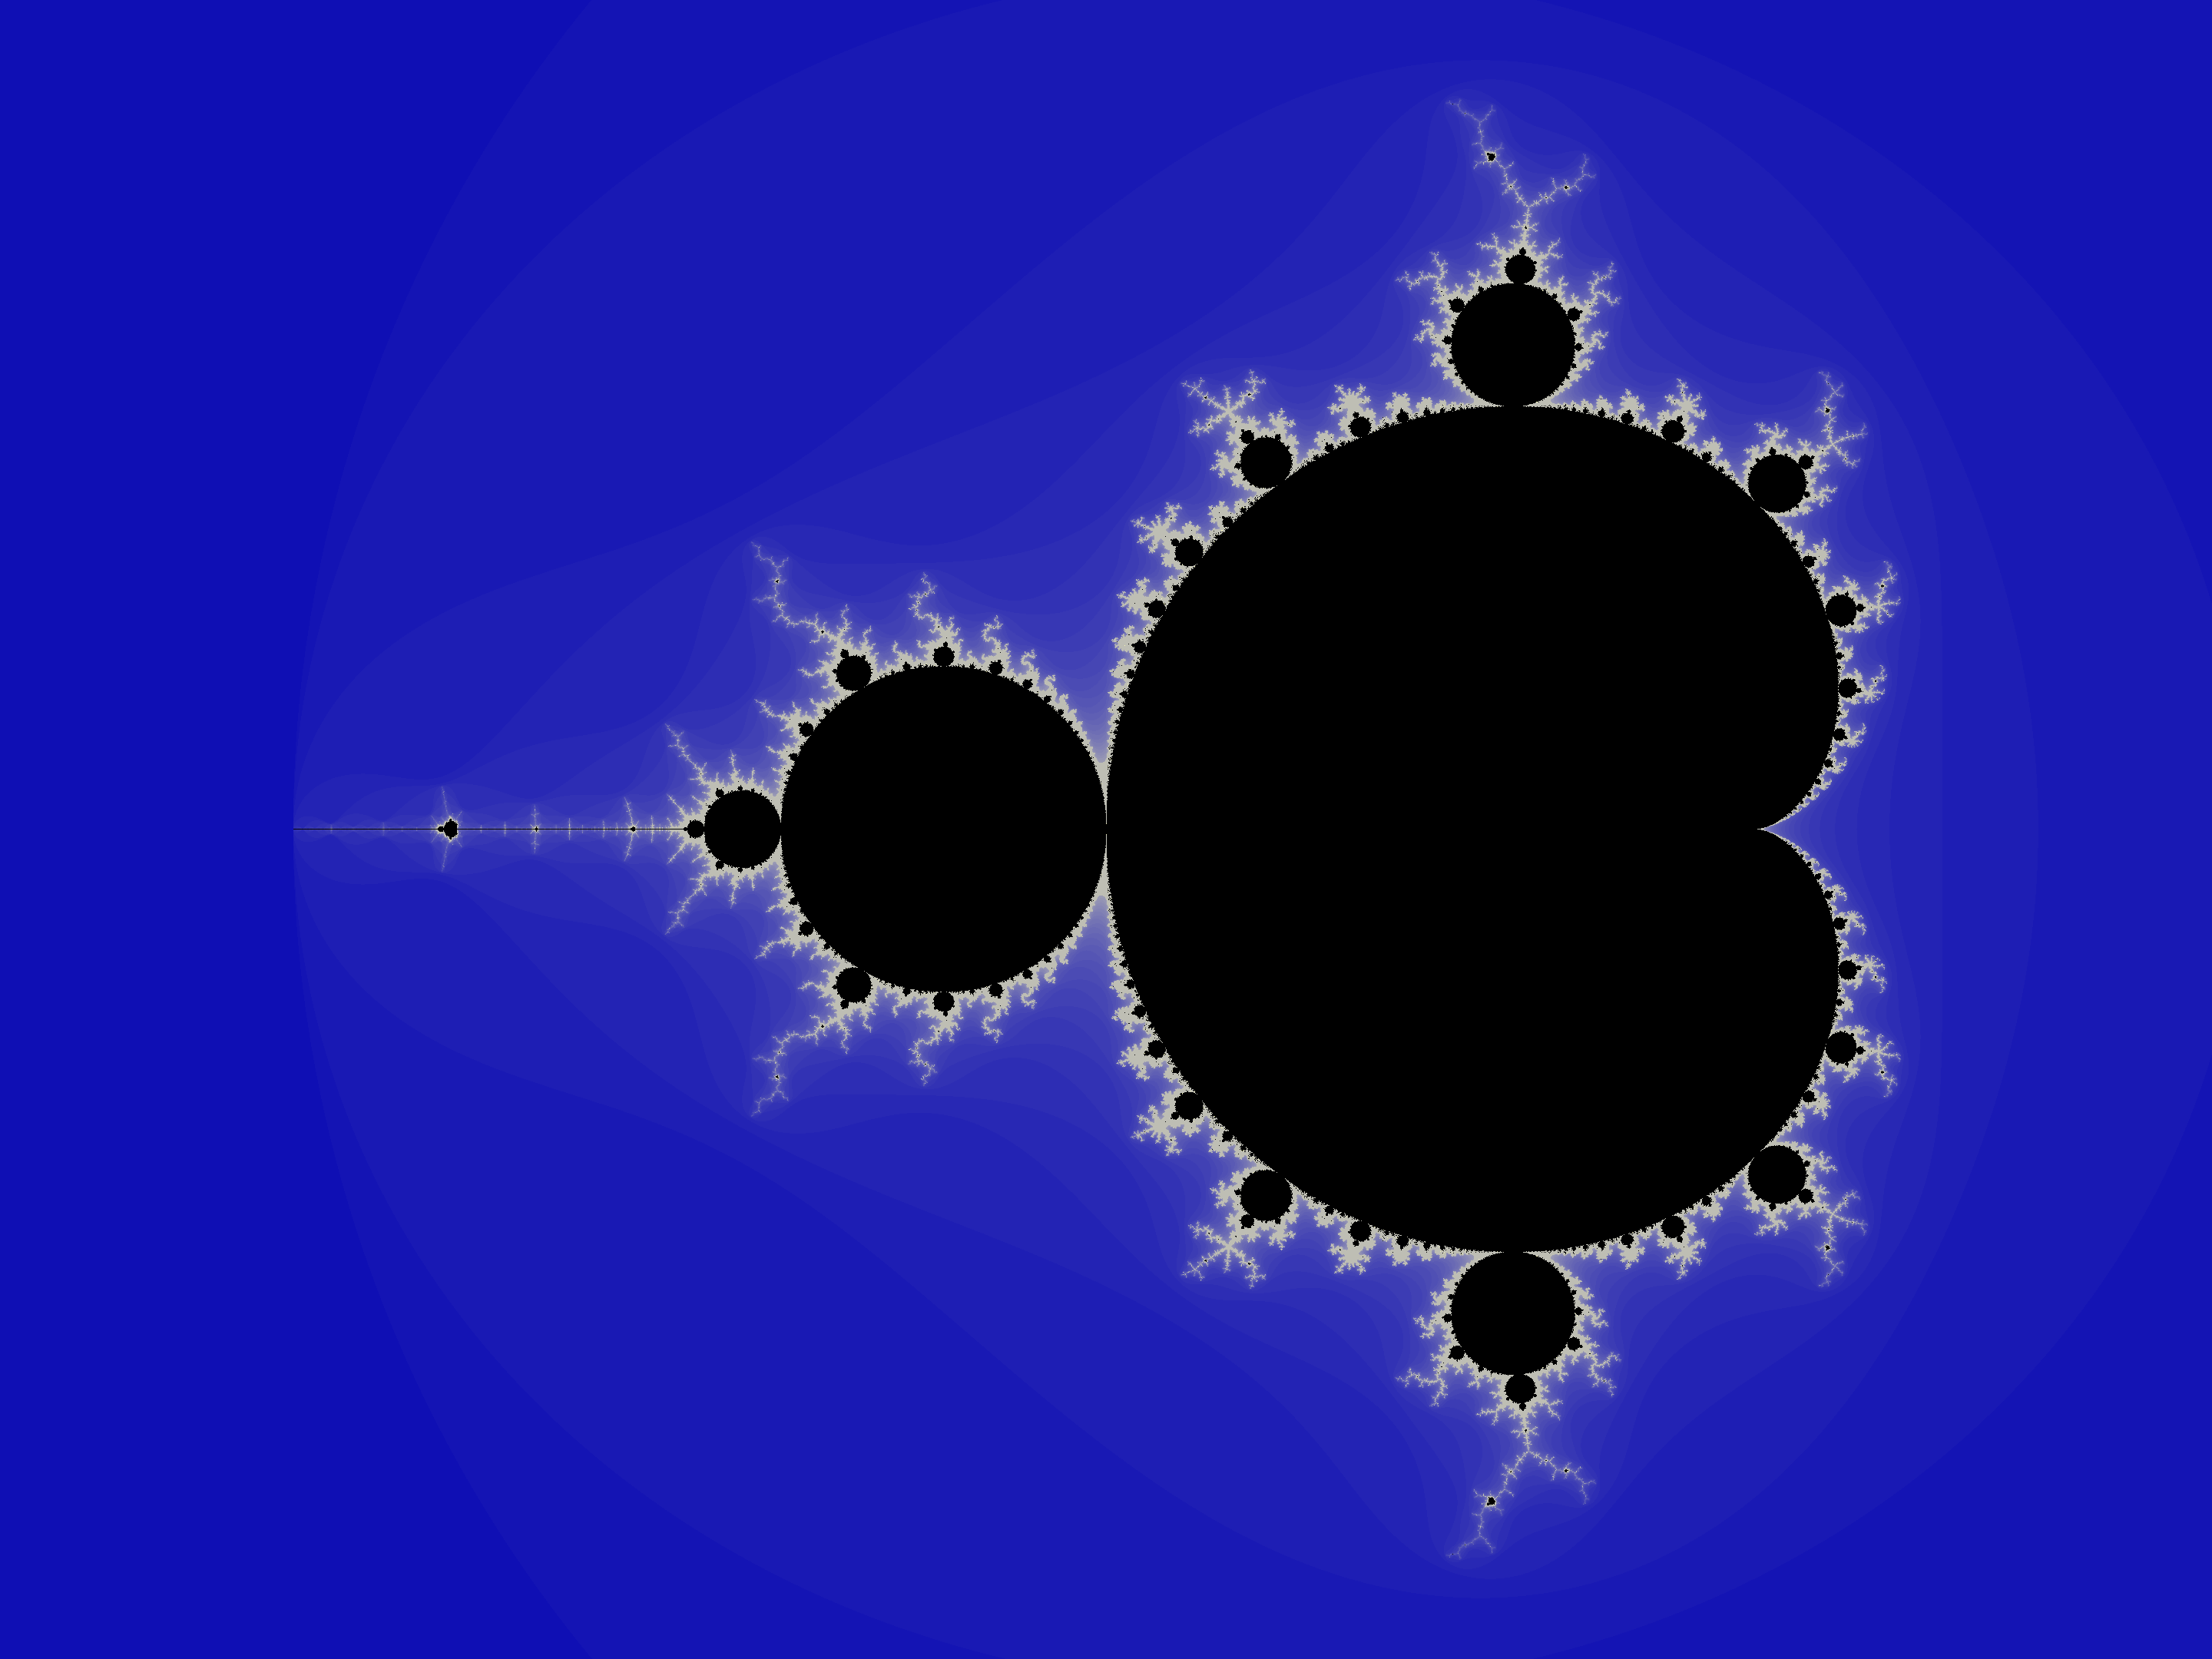
\includegraphics[width=8cm,height=6cm]{./examples/res_color_400.png}
\caption{\label{Two}}
\end{figure}

\section{结论}
\indent 由上边的图片,我们可以看到,随着迭代次数上限的提高,图像所展示的形状越趋向于真实的Mandelbrot Set ,但是在同一图片像素个数的前提下,随着 N 越来越大,继续提升 N 对于肉眼辨识下的图片提升已经不明显,像上边迭代上限400次和迭代上限5000次的图像相差并不大。
\bibliographystyle{IEEEtran}  %格式
\bibliography{./doc/example}
\end{document}